\chapter{Introduction}
\label{chp:introduction}

% Performance evaluation of software architectures:  http://dl.acm.org/citation.cfm?id=287353

% Experience with Performance Testing of Software Systems: Issues, an Approach, and Case Study: http://search.proquest.com/docview/195577700?pq-origsite=gscholar

% The Future of Software Performance Engineering: http://ieeexplore.ieee.org/xpls/abs_all.jsp?arnumber=4221619&tag=1

% Performance Regression Testing Target Prioritization via Performance Risk Analysis: http://opera.ucsd.edu/paper/icse14-perfscope.pdf

% 

Performance is a make-or-break quality for software.
In today's society we expect manufacturers to progress in their expertise and their products to advance.
We take for granted that new cars have a larger radius, are more powerful, less pollute and more safe with each iteration of design.
In contrast, software does not has this image; software updates breaking functionalities, adding severe performance issues or increasing the complexity of the user interface are common.
The Facebook mobile Android application is a prime example of this, having more than one billion installs and being in development for years by a complete development department, still receives updates which causes performance issues for users, see Figure~\ref{fig:facebook_bad_reviews}.
Just as with their cars users expect software performance to advance or at least not become \emph{worse}. 
Smith et al. have shown that the cost of a software product is determined more by how well it achieves its objectives for quality attributes such as performance than by its functionality \cite{smith2003software}.
This motivates items such as performance to be taken into consideration by both industry as academia when developing software.

\begin{figure}[h]
	\centering
	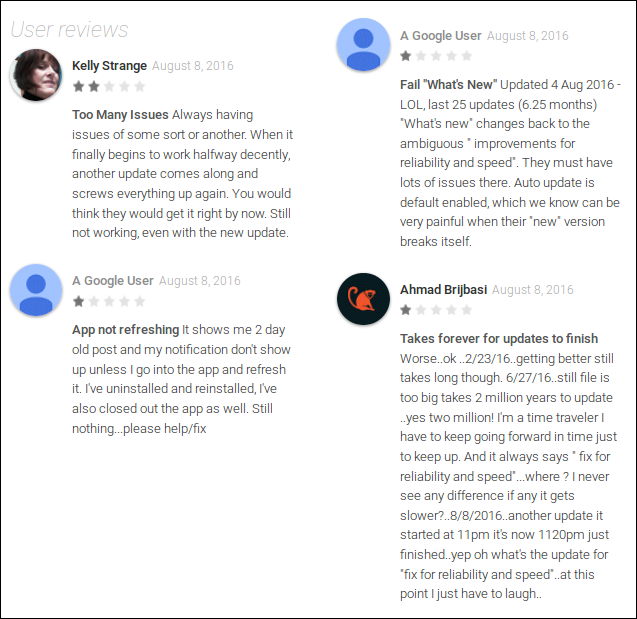
\includegraphics[width=\linewidth]{introduction/images/bad_reviews.png}
	\caption{Bad reviews showing the Facebook Android application introducing issues with updates.}
	\label{fig:facebook_bad_reviews}
\end{figure}

Performance can be divided in two dimensions: \emph{responsiveness} and \emph{scalability}.
Responsiveness is the ability of a system to meet the requirements for response time or throughput.
The response time can be measured by how fast a system can respond to an event, where throughput can be measured by how many events can be processed in a set amount of time.
Scalability is the ability of a system to meet the required response time or throughput when faced with a growing demand of its software functions.

Performance plays an important role in both industrial and academic areas.
For instance, an increase of 500 milliseconds latency in Google's search results could cause 20\% traffic loss \cite{mayer2009search}.  
The deterioration of performance introduced by changes is often referred to as \emph{performance regression}.
Performance regression can lead to several undesired consequences such as damaged customer relationships as the software does not meet its required performance.
Huang et al. provide the example of an e-commerce website that saw an increase of 2000\% in their page loading times because of an update to the underlying database engine \cite{huang2014performance}.
These situations can lead to lost revenue and possibly missed market windows.
Other consequences of performance failures may express themselves in lost productivity for users, increased costs, failures on deployment or even abandonment of projects \cite{woodside2007future, williams1998performance}.

To inspect whether the performance of a system has decreased, performance regression testing can be applied.
Using this method, the system is tested for performance regression under various loads \cite{woodside2007future}.
Traditional software development focusses on correctness, causing regression testing to be deferred to a late stage in the development cycle, if applied at all.
%This approach is often called the \enquote{fix-it-later} approach.
To illustrate the varying amounts of regression testing appliances, Huang et al. mention the performing testing interval of MySQL, Linux and Chrome.
These projects apply performance tests every release, every week and every four revisions, respectively.
Once performance regression is detected, developers have to spend extra efforts determining what causes said regression, especially when a lot of changes have been applied to the code base since the last measurement \cite{huang2014performance}.
Performance tests should be executed as frequently as possible, ideally per change made by developers.
However, as some tests take hours or even weeks, this approach is not always feasible.

\emph{Software performance engineering} (SPE) is the discipline concerned with constructing software systems that meet performance objectives \cite{smith2003best}.
It prescribes principles for creating responsive software, methods to obtain performance specifications and offers guidelines for the types of evaluations to be conducted at each development stage.
SPE features two general approaches \cite{woodside2007future} where the first approach is purely measurement based.
This characterizes itself by performing actions late in the development cycle such as  applying regression tests, diagnosis and tuning, when the system can be run and measured in real-time.
The second approach features a model-based style.
Using this approach, performance models are created at the early stages of development, influencing the architecture and design of the system to meet performance requirements.

\todo{Uitleggen dat performance in centralized architecturen makkelijker is te tunen dan een decentraal systeem + plaatje met verschil}.

\begin{figure}[!h]
	\centering
	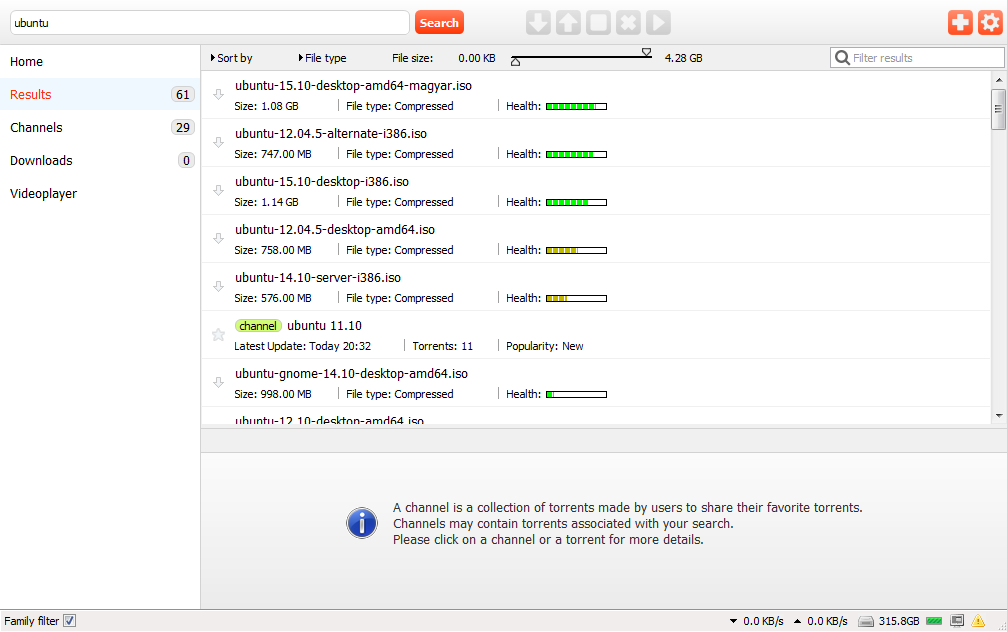
\includegraphics[width=\linewidth]{introduction/images/tribler_screenshot.png}
	\caption{Screenshot of Tribler v6.5.2.}
	\label{fig:tribler_screenshot}
\end{figure}

Tribler is the result of ten years of scientific research in the field of decentralized systems and online cooperation.
Over 100 scientific publications have Tribler in their foundation.
Tribler is completely open-source and can be downloaded from the Tribler website\footnote{\url{https://www.tribler.org}}.
Tribler's interface is visible in Figure~\ref{fig:tribler_screenshot}.\\
Over the course of more than a decade Tribler has gained a tremendous amount of attention in both media and academia.
It has been downloaded approximately 1.8 million times \cite{github2016releases} and has more than two thousand monthly active users.
This makes Tribler one of the research projects that allow researchers to run experimental code \enquote{in the wild} on a large scale.

One of Tribler's unique features is that it allows users to discover and exchange data in a complete decentralized way.
This introduces additional challenges compared to centralized solutions.

Using a centralized structure, heavy computations can be offloaded to servers which are often more powerful and more responsive than a consumer grade computer.
Once the result has been computed, it can be communicated back to the user at only the cost of the communication. 
It has been demonstrated that for devices with a finite power supply such as smartphones, this technique can be applied to save energy or to boost performance \cite{kumar2010cloud, kemp2010cuckoo}.

Decentralized systems such as Tribler do not have such servers present that can be offloaded to, restricting the area of computation to the device itself.
It is thus essential that the software performs well on heterogeneous devices, possibly facing challenging network conditions.

To enhance privacy and anonymity, support for anonymous downloads was introduced in 2014 by R. Plak \cite{plak2014anonymous} and R. Tanaskoski \cite{tanaskoski2014anonymous}.
In 2015, the support for anonymous seeding of torrents using Tor-like hidden services was added by R. Ruigrok \cite{ruigrok2015bittorrent}.
A trade-off has to be made by Tribler between the desired performance and the level of anonymity provided, as any additional layer of privacy comes with an increased number of cryptographic operations.

Not only anonymity impacts the overall performance of Tribler: architectural flaws introduced in the past have led to a decrease in performance today.
This manifests itself in users frequently reporting high system load, a non-responsive Graphical User Interface and low download speed.
Furthermore, Tribler is plagued with a high number of disk operations which has been known since 2013 \cite{pouwelse2014reduce}. 

The focus of this thesis is to improve Tribler's performance by making use of software performance engineering techniques in the late stages of the development cycle with a particular focus on the performance of disk operations and software regression testing.

The rest of this thesis is structured as follows.
Chapter~\ref{chp:problem-description} provides the problem description and the research questions this thesis attempts to answer.
Chapter~\ref{cpt:pythons_thread_model} explains the python threading model and why we observe performance issues with Tribler.
Chapter~\ref{cpt:experiments} presents experimental results of this work.
Finally, Chapter~\ref{cpt:conclusion_and_future_work} concludes this thesis and provides future work.
